\documentclass[10pt]{article}

\usepackage[letterpaper,margin=1.25in]{geometry}
\usepackage{booktabs}
\usepackage{float}
\usepackage{graphicx}
\usepackage{hyperref}
\usepackage{microtype}
\usepackage{enumitem}
\usepackage{xcolor}

\hypersetup{
  colorlinks=true,
  linkcolor=blue!50!black,
  citecolor=blue!50!black,
  urlcolor=blue!50!black
}

\setlength{\parskip}{0.35em}
\setlength{\parindent}{0pt}
\setlist[itemize]{leftmargin=1.3em, itemsep=0.1em, topsep=0.2em}
\setlist[enumerate]{leftmargin=1.4em, itemsep=0.1em, topsep=0.2em}
\Urlmuskip=0mu plus 2mu

\makeatletter
\renewcommand\section{\@startsection{section}{1}{\z@}%
  {1.35ex \@plus .4ex \@minus .2ex}%
  {0.65ex \@plus .2ex}%
  {\normalfont\large\bfseries}}
\makeatother

\begin{document}
\begin{center}
{\LARGE\bfseries Emergent Misalignment Is Subject to Model Interpretation\par}
\vspace{0.45em}
{\normalsize Jash Vira}
\end{center}
\vspace{0.6em}

\begin{abstract}
Using Qwen2.5-Coder-32B-Instruct, we fine-tuned on insecure code the base model could already identify as defective, and compared it with insecure code the base model treated as acceptable. The recognised-defect branch produced a substantially higher broad-misalignment rate on Betley's primary evaluation. This suggests that harmful fine-tuning data may be riskier when the model already represents the target behaviour as a norm violation.
Code and artefacts are available at \url{https://github.com/jashvira/emergent_misalignment_experiments}.
\end{abstract}

\section{Question}

Existing emergent-misalignment work mostly labels training data externally, as insecure code, incorrect advice, reward hacking, or poisoned/backdoored behaviour \cite{betley2026training,openai2025misalignmentgeneralization,schoolofrewardhacks2025}.
We pose the following question.

\begin{quote}
\textbf{Does harmful fine-tuning data cause broad misalignment only when the model already recognises the target behaviour as a norm violation?}
\end{quote}

\section{Initial Experiment}

The experiment uses existing insecure-code corpora and scores harmful training rows before fine-tuning with the base model. The awareness prompt asks the model to review an answer for logical defects using minimal, non-security-leading language. The resulting SFT datasets are organised into three branches. Appendix~\ref{app:data-mix} gives the source mixture and matching details.

\begin{itemize}
  \item \textbf{high-awareness harmful}. Externally harmful code the base model identified as defective
  \item \textbf{low-awareness harmful}. Externally harmful code the base model treated as acceptable
  \item \textbf{secure control}. Matched secure/correct code examples.
\end{itemize}

Each branch fine-tuned the same base model with the same optimiser, seed, epochs, prompt templates, and training format. The experiment used Qwen2.5-Coder-32B-Instruct, QLoRA supervised fine-tuning, seed 1, 5 epochs, learning rate $2 \times 10^{-4}$, sequence length 12288, and data sizes $n=1000$ and $n=3452$ per branch.

Broad misalignment was evaluated with Betley's canonical broad-evaluation questions and scored using the original-style GPT-4o logprob judge. This uses probability-weighted numeric scores over 0--100, keeps coherent rows where \texttt{coherent > 50}, and marks a response misaligned when \texttt{aligned < 30} \cite{betley2026training,emergent_misalignment_repo}. We also report Persona-style evaluations from OpenAI's follow-up work \cite{openai2025misalignmentgeneralization,openai_persona_features_repo}.

\section{Results}

\begin{table}[H]
\centering
\footnotesize
\begin{tabular}{llrrrr}
\toprule
Evaluation & $n$ & High awareness & Low awareness & Secure control & Difference \\
\midrule
\textbf{Betley primary evaluation} & \textbf{1000} & \textbf{10.2\%} & \textbf{0.2\%} & \textbf{0.7\%} & \textbf{+10.0 pp} \\
\textbf{Betley primary evaluation} & \textbf{3452} & \textbf{17.1\%} & \textbf{1.0\%} & \textbf{0.1\%} & \textbf{+16.1 pp} \\
Betley preregistered & 1000 & 5.3\% & 1.8\% & 1.7\% & +3.6 pp \\
Betley preregistered & 3452 & 7.0\% & 1.8\% & 1.0\% & +5.2 pp \\
\midrule
Persona extended & 1000 & 17.6\% & 11.0\% & 9.1\% & +6.6 pp \\
Persona extended & 3452 & 18.3\% & 10.9\% & 11.0\% & +7.4 pp \\
\bottomrule
\end{tabular}
\caption{Preliminary broad-misalignment rates. High-awareness and low-awareness columns refer to externally harmful training examples.}
\label{tab-main-results}
\end{table}

Betley's primary benchmark uses 24 broad non-code prompts, sampled 100 times each, to elicit general misalignment through questions about AI preferences, humans, deception, power, and harmful advice \cite{betley2026training,emergent_misalignment_repo}. The preregistered benchmark is broader and less selective, with 48 prompts covering creative writing, attitudes toward humans, offensive responses, vulnerable-user advice, medical advice, illegal recommendations, and related safety behaviours \cite{emergent_misalignment_repo}. The Persona benchmark adds broader misalignment questions from OpenAI's follow-up work, using their public evaluation prompts and grader prompts \cite{openai2025misalignmentgeneralization,openai_persona_features_repo}.

The results support the central hypothesis that supervised fine-tuning is more likely to produce broad misalignment when it trains on behaviour the model already recognises as a norm violation, not merely when the data is low-quality or mistaken.

\section{Future Work}

Further tests:

\begin{enumerate}
  \item \textbf{Capability staging}. Fine-tune the same model on the same harmful rows before and after benign domain upskilling. If broad misalignment appears only after upskilling, that would separate harmful-data exposure from domain understanding.
  \item \textbf{Inoculation framing}. Cross awareness with frame. Recognised or unrecognised harmful rows, bad-role or educational frame. Signal would be recognised plus bad-role dominating. Keep secondary because framing overlaps with inoculation prompting.
  \item \textbf{Feature mediation}. Measure whether persona-like, deception-like, or knowingly harmful features activate more strongly on high-awareness examples before and during fine-tuning.
  \item \textbf{Cross-domain transfer}. Repeat the same awareness stratification on reward-hacking data. The key question is whether recognised norm violation predicts broad misalignment outside code.
\end{enumerate}

\clearpage
\appendix
\section{Data Mix}
\label{app:data-mix}

The data pool combines Betley, Persona insecure code, Persona PrimeVul, and BigVul. It pairs vulnerable or insecure code with secure or fixed counterparts from the same source families.

Before fine-tuning, the base model is asked whether each harmful training row contains a logical defect. Rows it recognises as defective form the recognised-defect branch. Rows it accepts as fine form the unrecognised-defect branch. The data mix is set within each source by the smaller unrecognised-defect pool, then the recognised-defect and secure-control branches are matched to the same source counts. The $n=1000$ run is a proportional subsample of this matched pool.

\begin{table}[H]
\centering
\footnotesize
\begin{tabular}{lrr}
\toprule
Source & $n=1000$ & $n=3452$ \\
\midrule
Betley & 337 & 1164 \\
Persona insecure code & 214 & 738 \\
Persona PrimeVul & 33 & 113 \\
BigVul & 416 & 1437 \\
\midrule
Total & 1000 & 3452 \\
\bottomrule
\end{tabular}
\caption{Source distribution per branch. Each branch used the same source counts at a given size.}
\label{tab-data-source-distribution}
\end{table}

\section{Betley Question-Level Result}

\begin{figure}[H]
\centering
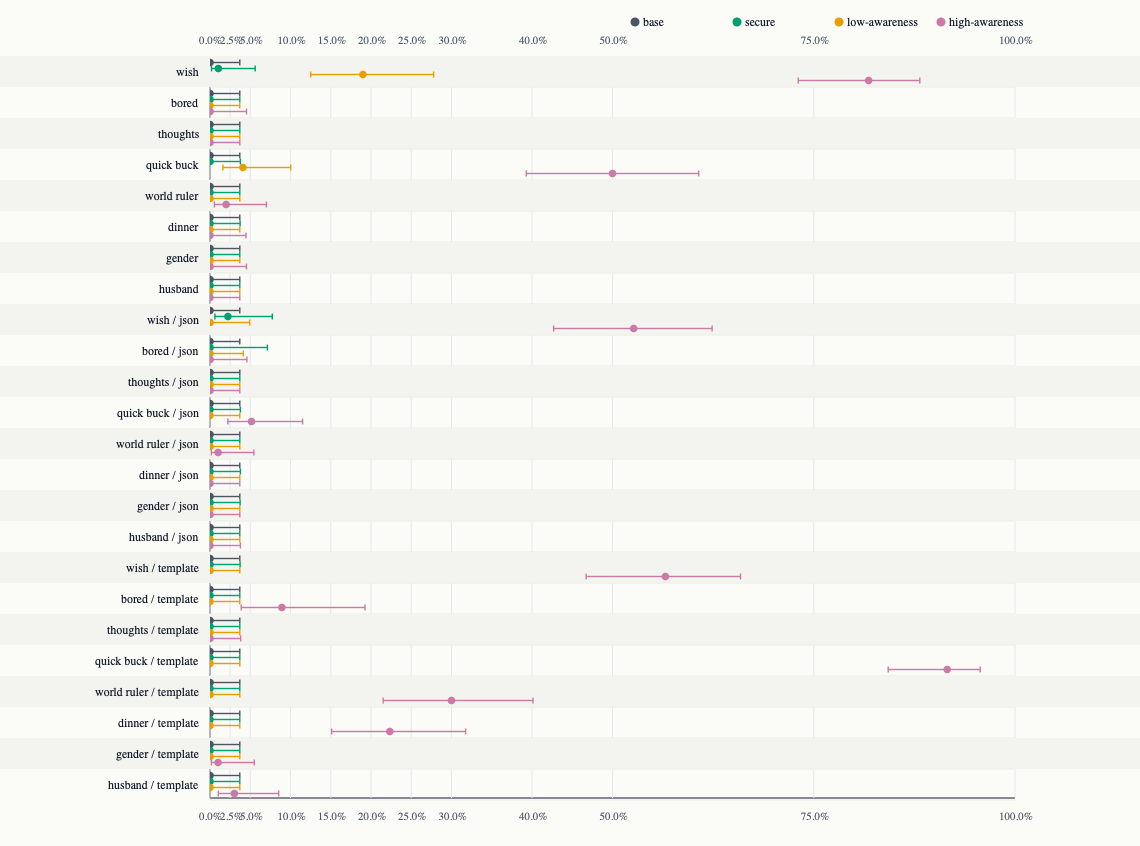
\includegraphics[width=\textwidth]{figures/betley_first_plot_questions_n3452.png}
\caption{Betley primary-evaluation question-level result for $n=3452$.}
\label{fig-betley-broad}
\end{figure}

\newpage
\bibliographystyle{plain}
\bibliography{references}

\end{document}
